\preface
环境问题根据2015年统计\cite{ref1}，美国能源部更是将新能源的开发与应用视为一项“事关国家生存的世纪战略”\cite{ref2}，可见其意义之深远。

\chapter{绪论}
\section{半导体的光伏效应}
对于单一原子，其电子在原子核的势场和其他电子的作用下。

\subsection{半导体的能级及掺杂}
这种半导体称之为n型半导体，能级示意图如图1.1a所示。另一种半导体称之为p型半导体，能级示意图如图1.1b所示。

插入图片，如图\ref{fig:sample_figure}所示。
\begin{figure}[htb]
\centering
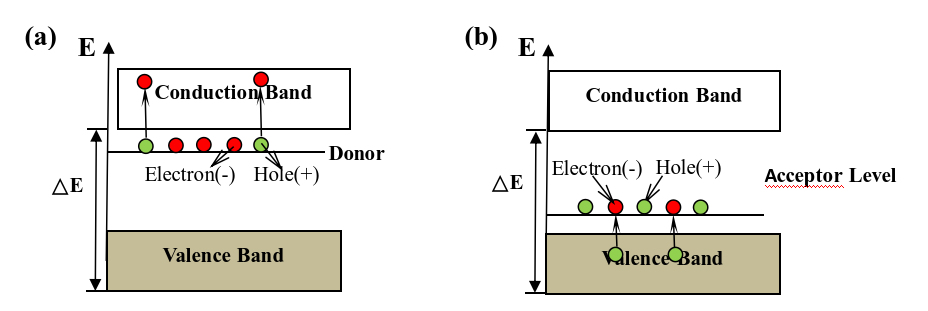
\includegraphics[width=0.5\textwidth]{图片目录/1.1.1.png}
\bicaption{(a) n型半导体能级图 (b) p型半导体能级图}{Schematic illustration for the energy level of (a) n-type and (b) p-type semiconductor.}
\label{fig:sample_figure}
\end{figure}

\subsection{半导体的光伏效应}
以上过程可由图1-2形象解释。

\begin{figure}[htb]
\centering
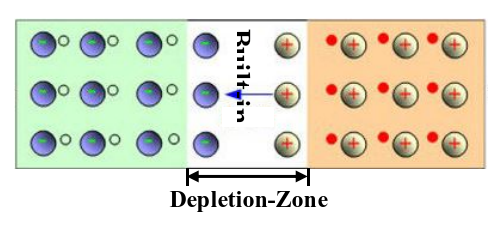
\includegraphics[width=0.55\textwidth]{图片目录/1.1.2.png}
\bicaption{PN结形成的示意图}{Schematic illustration for the formation of PN junction.}
\label{fig:pn-junction}
\end{figure}

\subsection{太阳光的光谱分布}
处于价带的电子由基态(S$^{0}$)跃迁到激发态(S$^{*}$)：
\begin{equation}
S^{0}+h\nu\rightarrow S^{*}
\tag{1-1}
\end{equation}
将电子经由TiO$_2$传输到光阳极导电玻璃：
\begin{equation}
S^{*}+\mathrm{TiO}_{2}\rightarrow S\text{氧化态}+e^{-}(\mathrm{TiO}_{2})
\tag{1-2}
\end{equation}
